%%% Lecture slides: what measurement did to a confidentiality-checker design.
%%% Style deliberately matches SPS_Final_LLVM_Confidentiality_Lecture.tex.
%%% Build: latexmk -pdf slides.tex

\documentclass[aspectratio=169,10pt]{beamer}

\usepackage[T1]{fontenc}
\usepackage{lmodern}
\usepackage{amsmath,amssymb,mathtools}
\usepackage{booktabs}
\usepackage{tikz}
\usetikzlibrary{arrows.meta,positioning,fit,shapes.misc}

\definecolor{Ink}{HTML}{172033}
\definecolor{Navy}{HTML}{183B56}
\definecolor{Blue}{HTML}{246BCE}
\definecolor{Teal}{HTML}{087E8B}
\definecolor{Orange}{HTML}{E87524}
\definecolor{Mist}{HTML}{EDF3F8}
\definecolor{Soft}{HTML}{F7F9FC}
\definecolor{Muted}{HTML}{53657A}

\setbeamercolor{normal text}{fg=Ink,bg=white}
\setbeamercolor{structure}{fg=Blue}
\setbeamercolor{frametitle}{fg=Navy,bg=white}
\setbeamercolor{title}{fg=Navy}
\setbeamercolor{subtitle}{fg=Muted}
\setbeamercolor{block title}{fg=white,bg=Navy}
\setbeamercolor{block body}{fg=Ink,bg=Mist}
\setbeamercolor{alerted text}{fg=Orange}
\setbeamertemplate{navigation symbols}{}
\setbeamertemplate{itemize item}{\color{Blue}$\blacktriangleright$}
\setbeamertemplate{itemize subitem}{\color{Teal}$\bullet$}
\setbeamertemplate{footline}{%
  \leavevmode\hbox{%
  \begin{beamercolorbox}[wd=.84\paperwidth,ht=2.5ex,dp=1.1ex,leftskip=1.2em]{author in head/foot}%
    \color{Muted}\scriptsize Confidentiality checking across compiler lowering -- what measurement changed
  \end{beamercolorbox}%
  \begin{beamercolorbox}[wd=.16\paperwidth,ht=2.5ex,dp=1.1ex,rightskip=1.2em plus1fil]{date in head/foot}%
    \color{Muted}\scriptsize\hfill\insertframenumber/\inserttotalframenumber
  \end{beamercolorbox}}}
\setbeamertemplate{frametitle}{\vspace{0.25em}\insertframetitle\par\vspace{-0.35em}\color{Blue}\rule{\textwidth}{0.6pt}}

\newcommand{\good}[1]{\textcolor{Teal}{\textbf{#1}}}
\newcommand{\bad}[1]{\textcolor{Orange}{\textbf{#1}}}
\newcommand{\code}[1]{\texttt{#1}}
\newcommand{\vs}{\textcolor{Muted}{$\rightarrow$}}

\title{The compiler is part of your threat model}
\subtitle{Building a confidentiality checker, and being wrong six times}
\author{Working notes}
\date{}

\begin{document}

% ---------------------------------------------------------------- title
\begin{frame}[plain]
  \titlepage
  \begin{center}
  \small\color{Muted}
  All measurements: clang / llc / mlir-opt 17.0.6, reproduced end to end.
  \end{center}
\end{frame}

% ---------------------------------------------------------------- the question
\begin{frame}{The question}
  Does this compiled artifact reveal a secret to someone not entitled to it?

  \vspace{1em}
  Some dependence on the secret is \emph{intended} --- a service returning nothing
  derived from its inputs is useless. So the property is release-relative:

  \begin{block}{}
  \[
    \forall p,s_0,s_1:\quad R(p,s_0)=R(p,s_1)\;\Longrightarrow\;
    \mathrm{Obs}_\Theta(\mathrm{Tr}(P,p,s_0))=\mathrm{Obs}_\Theta(\mathrm{Tr}(P,p,s_1))
  \]
  \end{block}

  \vspace{0.5em}
  The adversary picks the public inputs once and two secrets freely. If they can
  make \emph{any} observable differ while what they are entitled to stays equal,
  the program leaks.

  \vspace{0.5em}
  \bad{A violation is a pair of executions.} No single run is a counterexample.
\end{frame}

% ---------------------------------------------------------------- why not correctness
\begin{frame}{Why a verified compiler does not help}
  CompCert-style correctness says the target computes the same \emph{function}.
  That is a statement about one execution. Confidentiality is not.

  \vspace{0.8em}
  Every one of these preserves the computed function and destroys the property:
  \begin{itemize}
    \item a conditional move becomes a branch \vs{} the observer learns the condition
    \item a division is strength-reduced \vs{} different operations, different timing
    \item a secret-scrubbing store is eliminated \vs{} nothing read it
    \item an allocation size depends on a secret count
  \end{itemize}

  \vspace{0.8em}
  \good{Refinement preserves 1-safety for free. It does not preserve 2-safety.}
  Narrowing nondeterminism can turn two indistinguishable runs into two
  distinguishable ones.
\end{frame}

% ---------------------------------------------------------------- four outcomes
\begin{frame}{Four outcomes, and why three would be dishonest}
  \begin{center}
  \begin{tabular}{@{}l l l@{}}
  \toprule
  Outcome & Meaning & Obligations \\
  \midrule
  \good{verified}    & no residual forbidden dependence        & must be none \\
  \bad{unsafe}       & a leak, with a replayable witness       & must be none \\
  unknown            & required semantics or contract absent   & must name what is missing \\
  conditional        & correct if named assumptions hold       & must name every assumption \\
  \bottomrule
  \end{tabular}
  \end{center}

  \vspace{1em}
  The two middle values carry the weight. A two-valued tool must \emph{guess} at
  a function pointer, a recursive call, an opaque callee, a solver timeout --- and
  a guess toward \good{verified} is the failure that makes such a tool worthless.

  \vspace{0.5em}
  \code{unknown} is how it fails closed. \code{conditional} is how it stays honest
  about hardware facts no IR analysis can reach.
\end{frame}

% ---------------------------------------------------------------- laundering
\begin{frame}{The finding that reframed everything}
  A program written with an explicit secret branch:

  \begin{center}
  \begin{tabular}{@{}l l l@{}}
  \toprule
  & LLVM IR at \code{-O2} & x86-64 assembly \\
  \midrule
  written with a ternary          & \code{select}, no \code{br i1} & \bad{\code{je}} \\
  written with the CT mask idiom  & \emph{identical IR}            & \bad{\code{je}} \\
  mask $+$ \code{asm} barrier     & no \code{select}               & \good{branchless} \\
  \bottomrule
  \end{tabular}
  \end{center}

  \vspace{0.8em}
  \bad{leaky source \vs{} clean \code{-O2} IR \vs{} leaky binary}

  \vspace{0.5em}
  Mid-end speculation turns the branch into a select, which reads as a repair.
  \code{x86-cmov-converter} turns it back --- default-on, no profitability check on
  the memory path. \good{aarch64 emits \code{csel} and does not leak.}

  \vspace{0.5em}
  One artifact. Clean IR. Leaks on one target, safe on another.
\end{frame}

% ---------------------------------------------------------------- mask folding
\begin{frame}{The repair everyone writes does not work}
  \begin{block}{The standard constant-time blend}
  \code{return (v \& mask) | (x \& \textasciitilde mask);}
  \end{block}

  \vspace{0.6em}
  InstCombine recognises the intent and folds it \emph{back} into a \code{select}
  --- byte-identical IR to the version written with a ternary. The backend then
  branches on it.

  \vspace{0.8em}
  So the author wrote branchless code, the compiler understood the intent,
  converted it to the construct being avoided, and a later pass produced the
  branch being avoided.

  \vspace{0.8em}
  \bad{A corpus containing a ``fixed'' twin is not evidence that the repair works.}
  Only measuring the emitted code is.
\end{frame}

% ---------------------------------------------------------------- carriers
\begin{frame}{Every way of carrying policy downward leaks}
  \begin{center}
  \begin{tabular}{@{}l l@{}}
  \toprule
  Carrier & Measured failure \\
  \midrule
  MLIR \code{sps.*} attributes & \code{mlir-translate} drops all of them, silently \\
  LLVM metadata                & \code{combineMetadata} discards unknown kinds on merge \\
  parameter attributes         & dropped by every signature-changing pass \\
  opaque marker call           & no definition \vs{} no link; definition \vs{} inlined away \\
  debug info                   & explicitly non-semantic; may be dropped \\
  \bottomrule
  \end{tabular}
  \end{center}

  \vspace{0.8em}
  They are all attempts to make a \emph{policy fact} travel through a pipeline
  whose passes are obliged to preserve only semantics.

  \vspace{0.5em}
  \good{The pipeline is not misbehaving. It was never told these facts mattered.}
\end{frame}

% ---------------------------------------------------------------- marker
\begin{frame}{Marking a declassifier: what survives}
  Split the policy from the implementation. The hash inlines freely; a marker on
  the \emph{result} carries the release identity.

  \vspace{0.6em}
  First attempt --- an opaque function --- \bad{fails structurally}:
  a declaration must link, and the moment its definition is co-visible,
  attribute inference deduces \code{returned}, the optimizer rewrites uses,
  and the release edge is severed \emph{while the marker sits there decoratively}.

  \begin{block}{What works: tied-register inline asm --- no symbol at all}
  \code{\%h = call T asm sideeffect "// sps.declassify id=\$2",}\\
  \hspace*{2.2em}\code{"=r,0,i,\textasciitilde\{memory\}"(T \%raw, i32 <ID>)}
  \end{block}

  \vspace{0.4em}
  Nothing to define, link, or import. Survives \code{O1}--\code{Oz}, \code{lto},
  \code{thinlto}. \good{Zero machine cost} (9 instructions vs 9). A non-constant
  id is a \good{hard instruction-selection error}.
\end{frame}

% ---------------------------------------------------------------- inversion
\begin{frame}{If policy cannot go down, send observations up}
  \begin{center}
  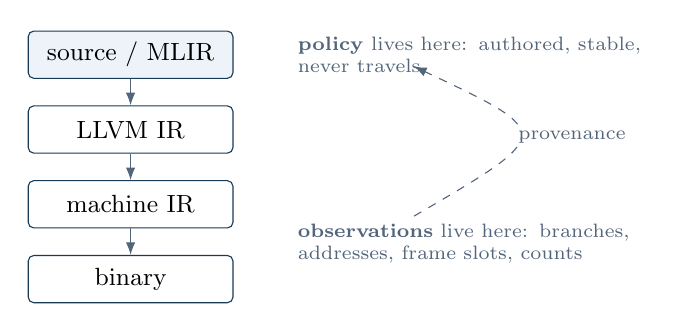
\begin{tikzpicture}[
    lvl/.style={draw=Navy, rounded corners=2pt, minimum height=6mm,
                minimum width=26mm, font=\small, inner sep=2pt},
    lbl/.style={font=\scriptsize, color=Muted},
    ar/.style={-{Latex[length=1.6mm]}, color=Muted}]
    \node[lvl, fill=Mist] (src) at (0,2.0)  {source / MLIR};
    \node[lvl]            (ir)  at (0,1.05) {LLVM IR};
    \node[lvl]            (mir) at (0,0.1)  {machine IR};
    \node[lvl]            (bin) at (0,-0.85){binary};
    \draw[ar] (src)--(ir); \draw[ar] (ir)--(mir); \draw[ar] (mir)--(bin);
    \node[lbl, anchor=west, text width=4.6cm] at (2.0,2.0)
      {\textbf{policy} lives here: authored, stable, never travels};
    \node[lbl, anchor=west, text width=4.6cm] at (2.0,-0.4)
      {\textbf{observations} live here: branches, addresses, frame slots, counts};
    \draw[ar, dashed] (3.6,-0.05) .. controls (5.4,1.0) .. (3.6,1.85);
    \node[lbl, anchor=west] at (4.8,0.95) {provenance};
  \end{tikzpicture}
  \end{center}

  \vspace{0.3em}
  \good{Level gap closes} --- observations gathered where they are real.\\
  \good{Annotation gap closes} --- labels never travel, so nothing can drop them.\\
  \good{Counting gap closes} --- cardinality measured, not asserted.
\end{frame}

% ---------------------------------------------------------------- quantifier
\begin{frame}{\dots and that design was wrong too}
  The first version said: \emph{for each policy site, check the predicate over the
  observations attributed to it}.

  \vspace{0.6em}
  That quantifies \bad{existentially over sites}. Soundness needs
  \good{universal quantification over observations}.

  \begin{block}{Why it matters}
  A per-site predicate cannot distinguish ``no observation here'' from
  ``compliant here''. Anything that moves an observation off a named site ---
  outlining, misattribution, a build without \code{-g} --- leaves an empty site
  that reads as compliance. \bad{It fails open, silently.}
  \end{block}

  \vspace{0.4em}
  \good{Universal discharge:} every policy-relevant observation must be discharged
  by exactly one site. Measured cost: 167 of 168 builds admissible.

  \vspace{0.4em}
  \emph{Same mistake one level down} --- the first fix rested soundness on the
  site namespace, which the compiler is equally free to rewrite.
\end{frame}

% ---------------------------------------------------------------- refusal
\begin{frame}{Then measure it on real code}
  \code{sqlite3.c}, 647 functions, \code{-O2 -g}:

  \begin{center}
  \begin{tabular}{@{}l r@{}}
  \toprule
  Operations lacking a source location & \good{4.80\%} \\
  Functions containing at least one    & \bad{62.9\%} \\
  \bottomrule
  \end{tabular}
  \end{center}

  \vspace{0.8em}
  The fixture corpus said $\approx$1\%. It averages \emph{seven} operations per
  fixture; real functions have \emph{eighty-nine}. The corpus could never have
  shown this.

  \vspace{0.6em}
  \bad{Refusal granularity is the defect}, not provenance quality:
  49\% of the refusals are functions missing \emph{one or two} locations out of 89.

  \vspace{0.5em}
  \emph{Caveat, stated plainly:} there is no policy here, so every operation was
  counted as relevant. This is the worst case, not a prediction.
\end{frame}

% ---------------------------------------------------------------- what exists
\begin{frame}{What actually exists}
  \begin{center}
  \begin{tabular}{@{}l r l@{}}
  \toprule
  Artifact & Size & Kind \\
  \midrule
  MLIR fixtures, C provenance, examples & $\sim$104 & test data \\
  \code{check\_harness.py}              & 929 & metadata validation \\
  \code{refusal\_rate.py}               & 179 & a scanner over IR text \\
  \code{sps-scan.cpp}                   & \good{174} & \good{an actual analysis} \\
  \bottomrule
  \end{tabular}
  \end{center}

  \vspace{1em}
  Of 1{,}320 lines of code, \good{174} implement an information-flow analysis.
  Everything else validates, measures, or documents.

  \vspace{0.8em}
  \bad{``The architecture refuses 63\% of functions''} is a claim about a system.\\
  \good{``63\% of functions contain an operation with no source location''} is what
  was measured.
\end{frame}

% ---------------------------------------------------------------- sps-scan
\begin{frame}{Running the 174 lines against the corpus}
  \begin{center}
  \begin{tabular}{@{}l l@{}}
  \toprule
  Group & Result \\
  \midrule
  \good{Caught correctly}       & the predecessor-choice countermodel; prefix-causal release \\
  \good{Silent correctly}       & five fixtures at zero --- a blanket-unsafe pass fails here \\
  \good{Imprecise as predicted} & the two controls that \emph{must} lose precision \\
  \bad{Missed, known reasons}   & audience, release-conformance, helper latency \\
  \bottomrule
  \end{tabular}
  \end{center}

  \vspace{1em}
  The two firing controls are \emph{not} a defect. Those fixtures exist to
  document that a forward \textsf{Low}/\textsf{High} lattice must lose precision
  there, and each declares \code{l1 disposition: relational-required}.

  \vspace{0.5em}
  \good{First time a prediction in this work was confirmed by running something}
  rather than by argument.
\end{frame}

% ---------------------------------------------------------------- six for six
\begin{frame}{Six claims, six corrections --- all by execution}
  \begin{center}
  \small
  \begin{tabular}{@{}p{0.44\textwidth} p{0.46\textwidth}@{}}
  \toprule
  Claim & Corrected by \\
  \midrule
  whole-run release equality as the product's initial constraint
    & the spec forbids it; unsound in the \emph{permissive} direction \\
  the marker as an opaque function
    & \code{returned} inferred once the definition is co-visible \\
  per-site quantification in the decision
    & a build verified under it, refused under universal discharge \\
  a register-only laundering reduction
    & did not reproduce; needs a memory operand \\
  an arithmetic-mask repair
    & folded back to a select, identical to the leaky twin \\
  a refusal surface of $\approx$1\%
    & 4.8\% per observation, 63\% per function \\
  \bottomrule
  \end{tabular}
  \end{center}

  \vspace{0.6em}
  None was caught by review, internal consistency, or re-reading the spec.
  \bad{A design claim that has not been executed is not evidence.}
\end{frame}

% ---------------------------------------------------------------- next
\begin{frame}{The smallest useful next step}
  \code{sps-scan} is not referenced anywhere in the harness. Wiring it in turns
  the corpus from a specification into a test of an implementation.

  \begin{enumerate}
    \item Add it to the diagnostic \code{RUN} of the satisfiable gates \vs{}
          real false-negative measurement
    \item Add it to the four precision controls \vs{} \good{the first
          false-positive net the corpus has ever had}
    \item Re-derive the refusal number from the analysis, with a real policy
  \end{enumerate}

  \vspace{0.8em}
  None of this needs the lowering architecture, the \code{.ll}-versus-MLIR
  decision, or the thirty unmigrated fixtures. Those gate \emph{later} layers.
\end{frame}

% ---------------------------------------------------------------- takeaway
\begin{frame}{Takeaways}
  \begin{itemize}
    \item \good{The compiler is inside the threat model.} Leaky source, clean IR,
          leaky binary is reproducible with default flags.
    \item \good{Durable mechanisms ask for nothing.} The inline-asm marker works
          because it is opaque by construction, not by permission.
    \item \good{Refusal granularity is a soundness \emph{and} usability decision.}
          Per-function turns 4.8\% into 63\%.
    \item \good{Corpus size determines what a corpus can tell you.} Seven
          operations per fixture cannot predict eighty-nine.
    \item \bad{The architecture was rewritten twice in a day.} What survived was
          the reproduced compiler behaviours, the fixtures, and the scripts.
  \end{itemize}

  \vspace{0.6em}
  \begin{block}{}
  \centering
  A design that cannot yet be executed should be weighted accordingly ---
  including this one.
  \end{block}
\end{frame}

\end{document}
